\section{Finite Difference Time Domain}
Finite Difference Time Domain (FDTD) is a very computationally intensive way to simulate the propagation of electromagnetic radiation.  It solves full on Maxwell's equations in time domain making no assumptions.  This approach has only been possible in the last few years with the increase in computing power.

Food for thought: Before using FDTD, you should be aware that in many cases when simulating a device, using FDTD is like using a sledge hammer to crack a nut.  For example when simulating a standard solar cell, one could use FDTD, this would involve simulating a wave front entering the cell through the top contact in time domain and waiting until the optical field reaches steady state then calculating how much light is being absorbed. This would require thousands of time domain simulation steps per wavelength.  However usually one is not interested in the time evolution of light in a solar cell as sunlight varies very slowly indeed, so one is better off not using a steady state method but other methods which assume light has already reached steady state, such as the transfer matrix method discussed above.

Never the less, FDTD is an import method, and can be used to design and understand complex devices.

Related YouTube videos:
\begin{figure}[H]

\begin{tabular}{ c l }


\includegraphics[width=0.05\textwidth]{./images/youtube.png}

&
\href{https://www.youtube.com/watch?v=il4Asw4-yQQ}{Generating photonic crystal structures for FDTD simulation}\
\\

\includegraphics[width=0.05\textwidth]{./images/youtube.png}

&
\href{https://www.youtube.com/watch?v=cnd5VRK56YM}{Tutorial on simulating photonic crystal waveguides using FDTD}

\end{tabular}
\end{figure}



\subsection{Running an FDTD simulation}
There is a demo FDTD simulation in the new simulations window. To open this click on new simulation in the file ribbon of the main window. The window in figure \ref{fig:fdtdnewdemo} will appear. Double click on the "Photonic-xtal FDTD" simulation to open it.  Save the simulation on your local hard disk, don't save it on a remote disk, USB disk or OneDrive they will be too slow to run the simulation.

\begin{figure}[H]
\centering
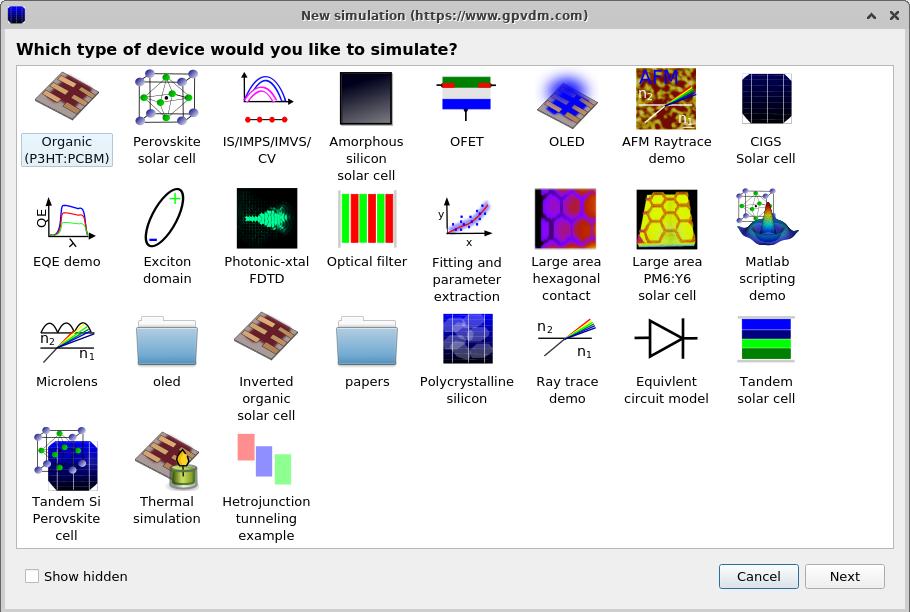
\includegraphics[width=0.7\textwidth]{./images/fdtd_1.png}
\caption{The new simulation window}
\label{fig:fdtdnewdemo}
\end{figure}

Once you have opened the simulation you should get a window which appears figure \ref{fig:fdtdfirstwindow}. If you click on the play button the FDTD simulation will run, it will take around 30 seconds to run.

\begin{figure}[H]
\centering
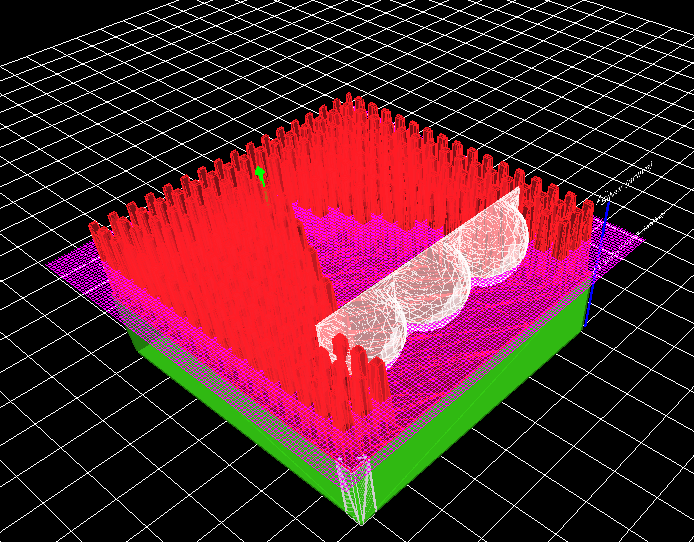
\includegraphics[width=0.7\textwidth]{./images/fdtd_2.png}
\caption{The initial FDTD simulation window. Use the slider to look at the results in time domain, and the drop down menu to select which field you are going to look at.}
\label{fig:fdtdfirstwindow}
\end{figure}

After the simulation has run click on the \emph{Output} tab and \ref{fig:fdtdoutputs} you will see the FDTD \emph{snapshots} folder, this can be seen in figure \ref{fig:fdtdoutputs}.  If you double click on this the FDTD snapshots window will appear which is shown in figure \ref{fig:fdtdsnapshots}.  This window will allow you to step through the simulations. If you click in the files to plot box, you will be able to select which field you plot. You will be able to select the \emph{Ey}, \emph{Ex} or \emph{Ez} fields.  In this case select the Ey field. Then use the slider bar to step through the field as a function of time.

\begin{figure}[H]
\centering
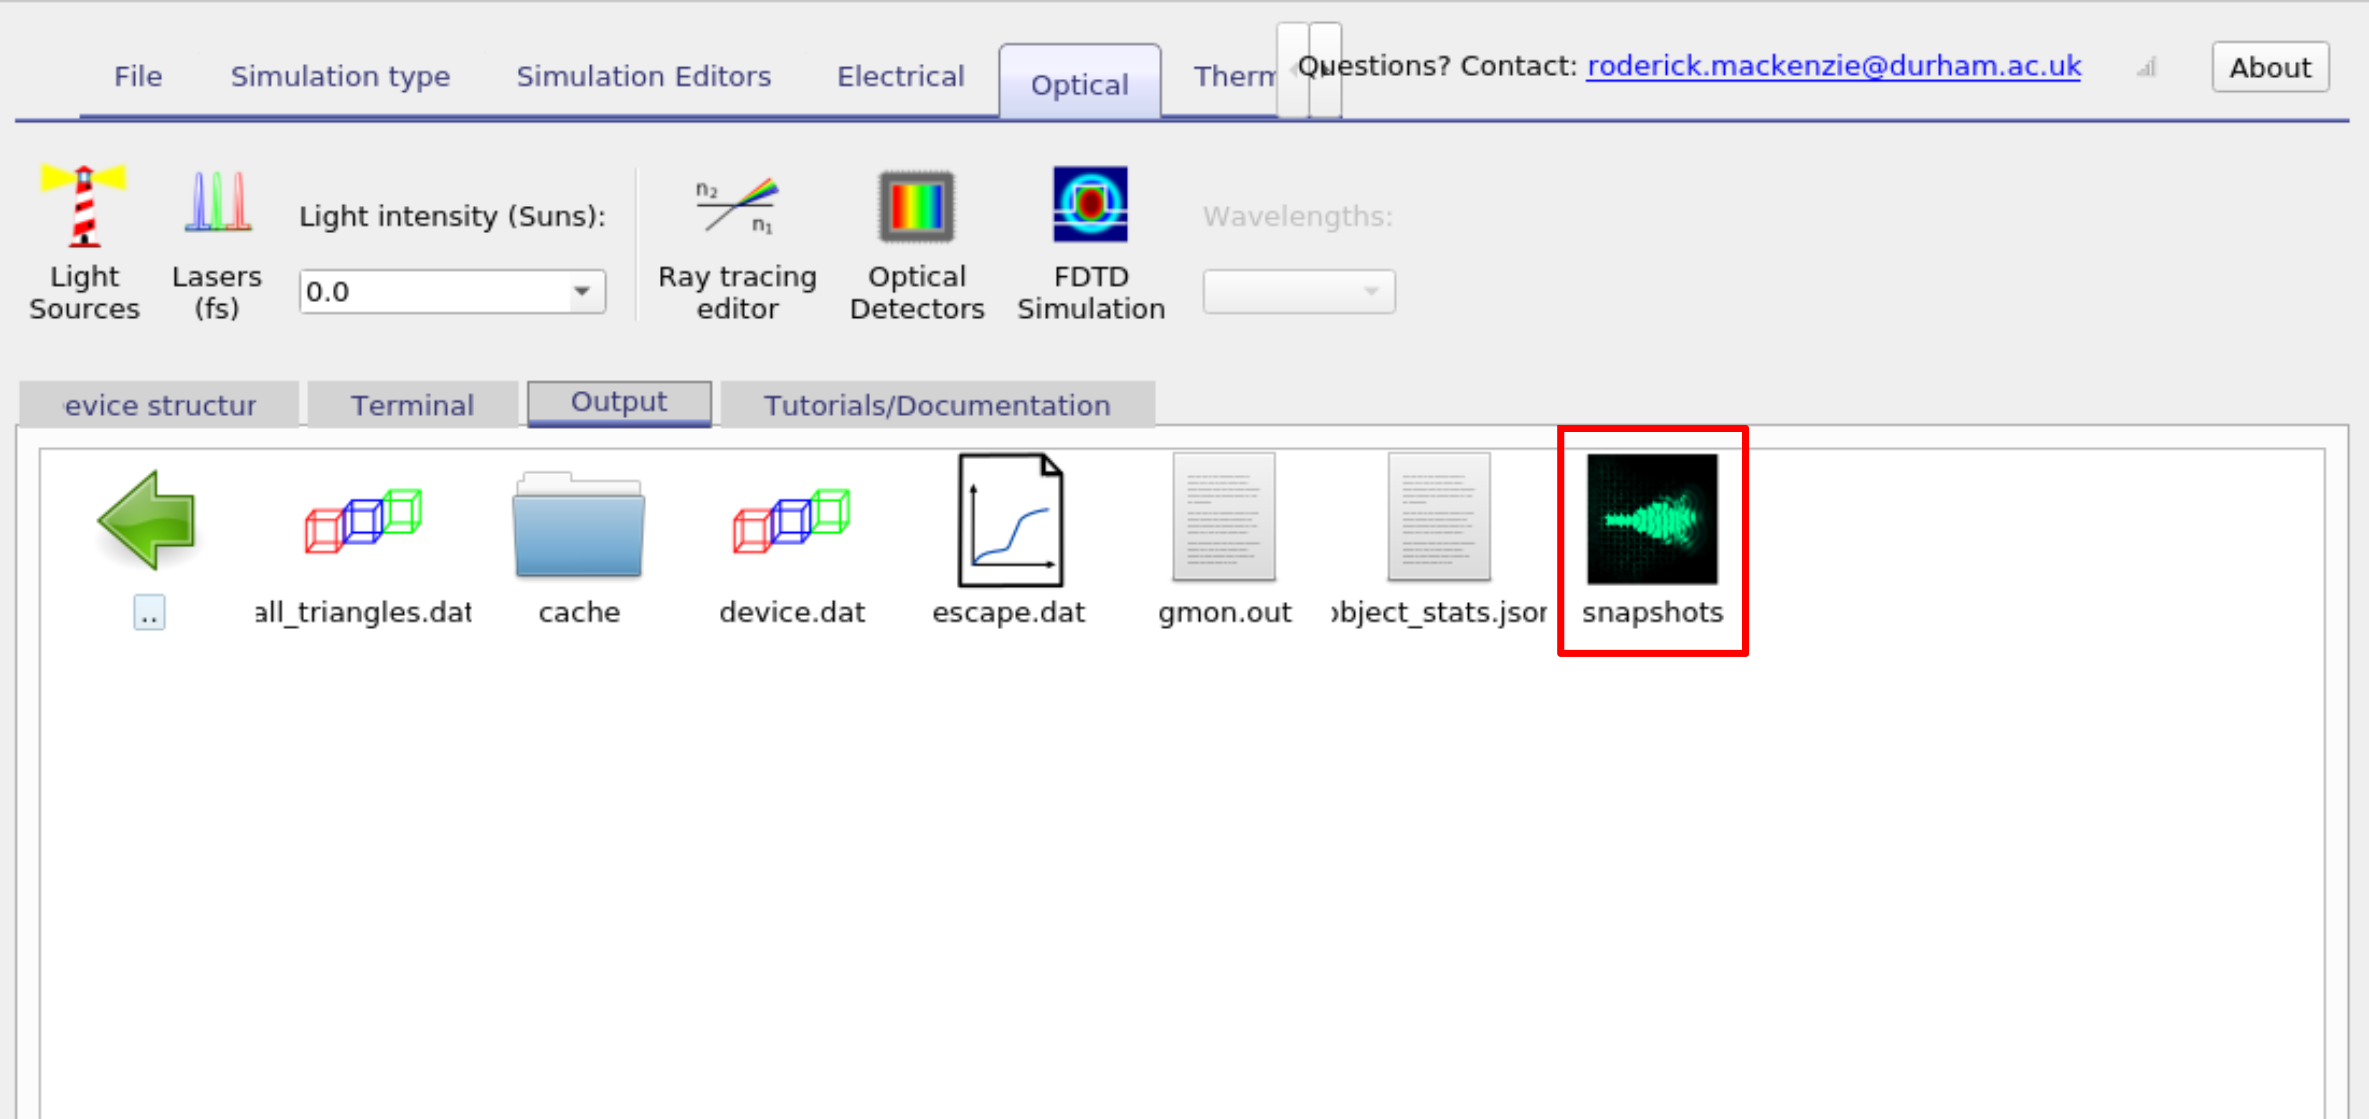
\includegraphics[width=0.7\textwidth]{./images/fdtd_8.png}
\caption{The output tab after having run an FDTD simulation, the key output is the Snapshots folder where the fields are stored.}
\label{fig:fdtdoutputs}
\end{figure}

\begin{figure}[H]
\centering
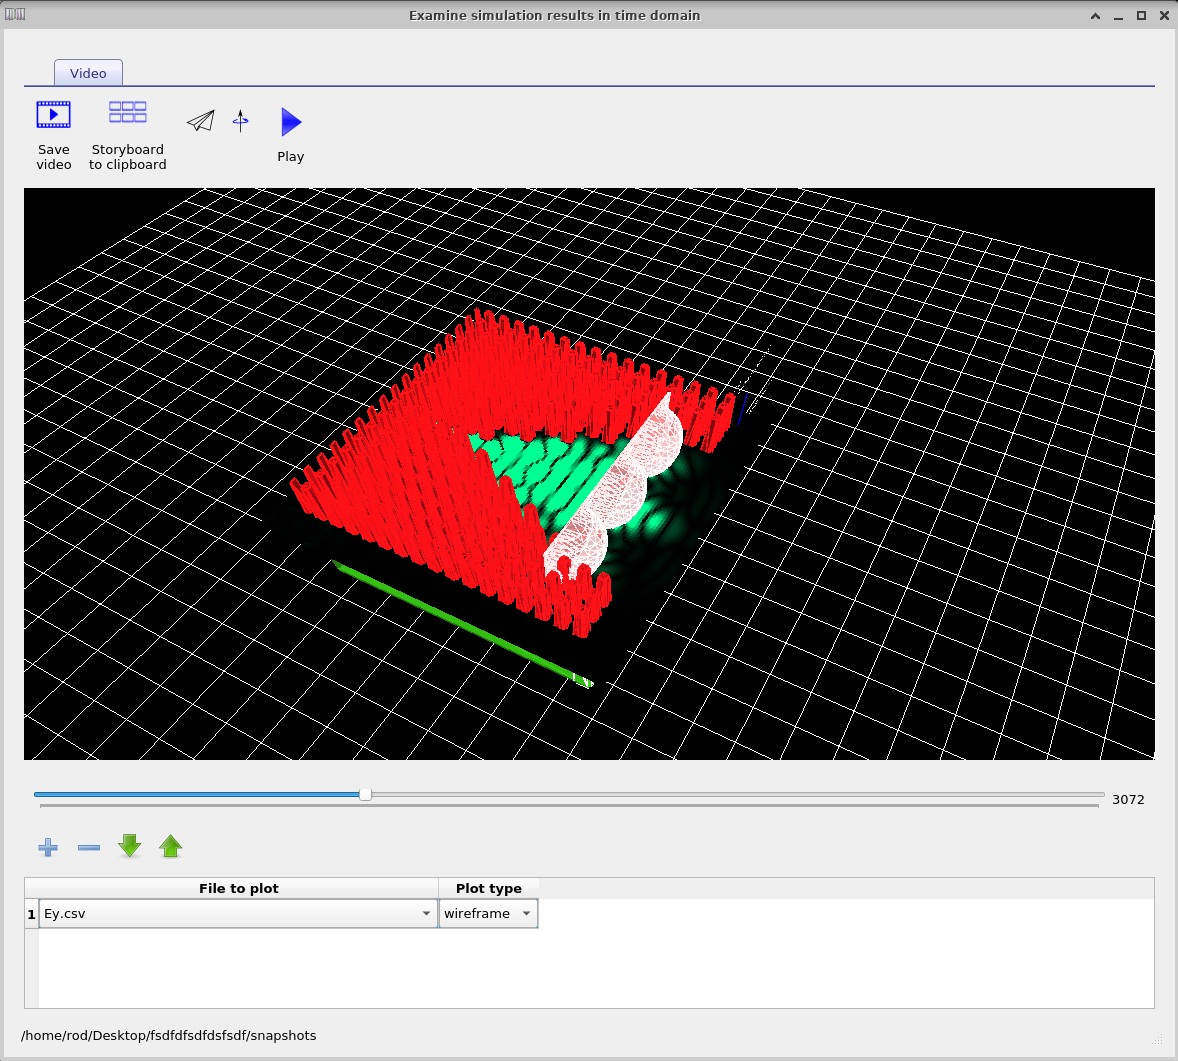
\includegraphics[width=0.7\textwidth]{./images/fdtd_9.png}
\caption{The FDTD snapshots window.}
\label{fig:fdtdsnapshots}
\end{figure}

\subsection{Manipulating objects in gpvdm}
Now close the snapshot viewer and go back to the main simulation window and select the \emph{Device tab}.  On the left of the window, you will see four buttons \emph{xy}, \emph{yz}, \emph{xz} and for little square boxes this can be seen in figure \ref{fig:fdtdmainwindow}. Try clicking them to see what happens to the view of the device.  After you have had a play select the \emph{xz} option, so that the screen looks like the left hand side of \ref{fig:fdtdmovingobjects}.  If you left click on the lenses, you will notice that you will be able to move them around. Try to move the lenses back in the device so that your device looks more like the right hand side of figure \ref{fig:fdtdmainwindow}.  If you hold shift down while dragging an object you can rotate it on the spot.

If you right click on the lenses and select \emph{Edit} you will be able to bring up the object Editor.  This shows the user all the object properties, this is visible in figure \ref{fig:objectviewer}. Try changing the object type from $convex\_lens$ to $concave\_ lens$ by clicking the edit button and rerunning the simulation.  If you want to add your own shapes to the shape data base see section \ref{sec:shapedatabase}. Using this window you can also change the material which is used in the FDTD simulation, the color of the object as well as its position or rotational angle.

The \emph{shape enabled} button enables you to turn off the shape if you don't want it in the simulation. If this shape were also electrically active you could also use this window to configure the electrical parameters.

 
\begin{figure}[H]
\centering
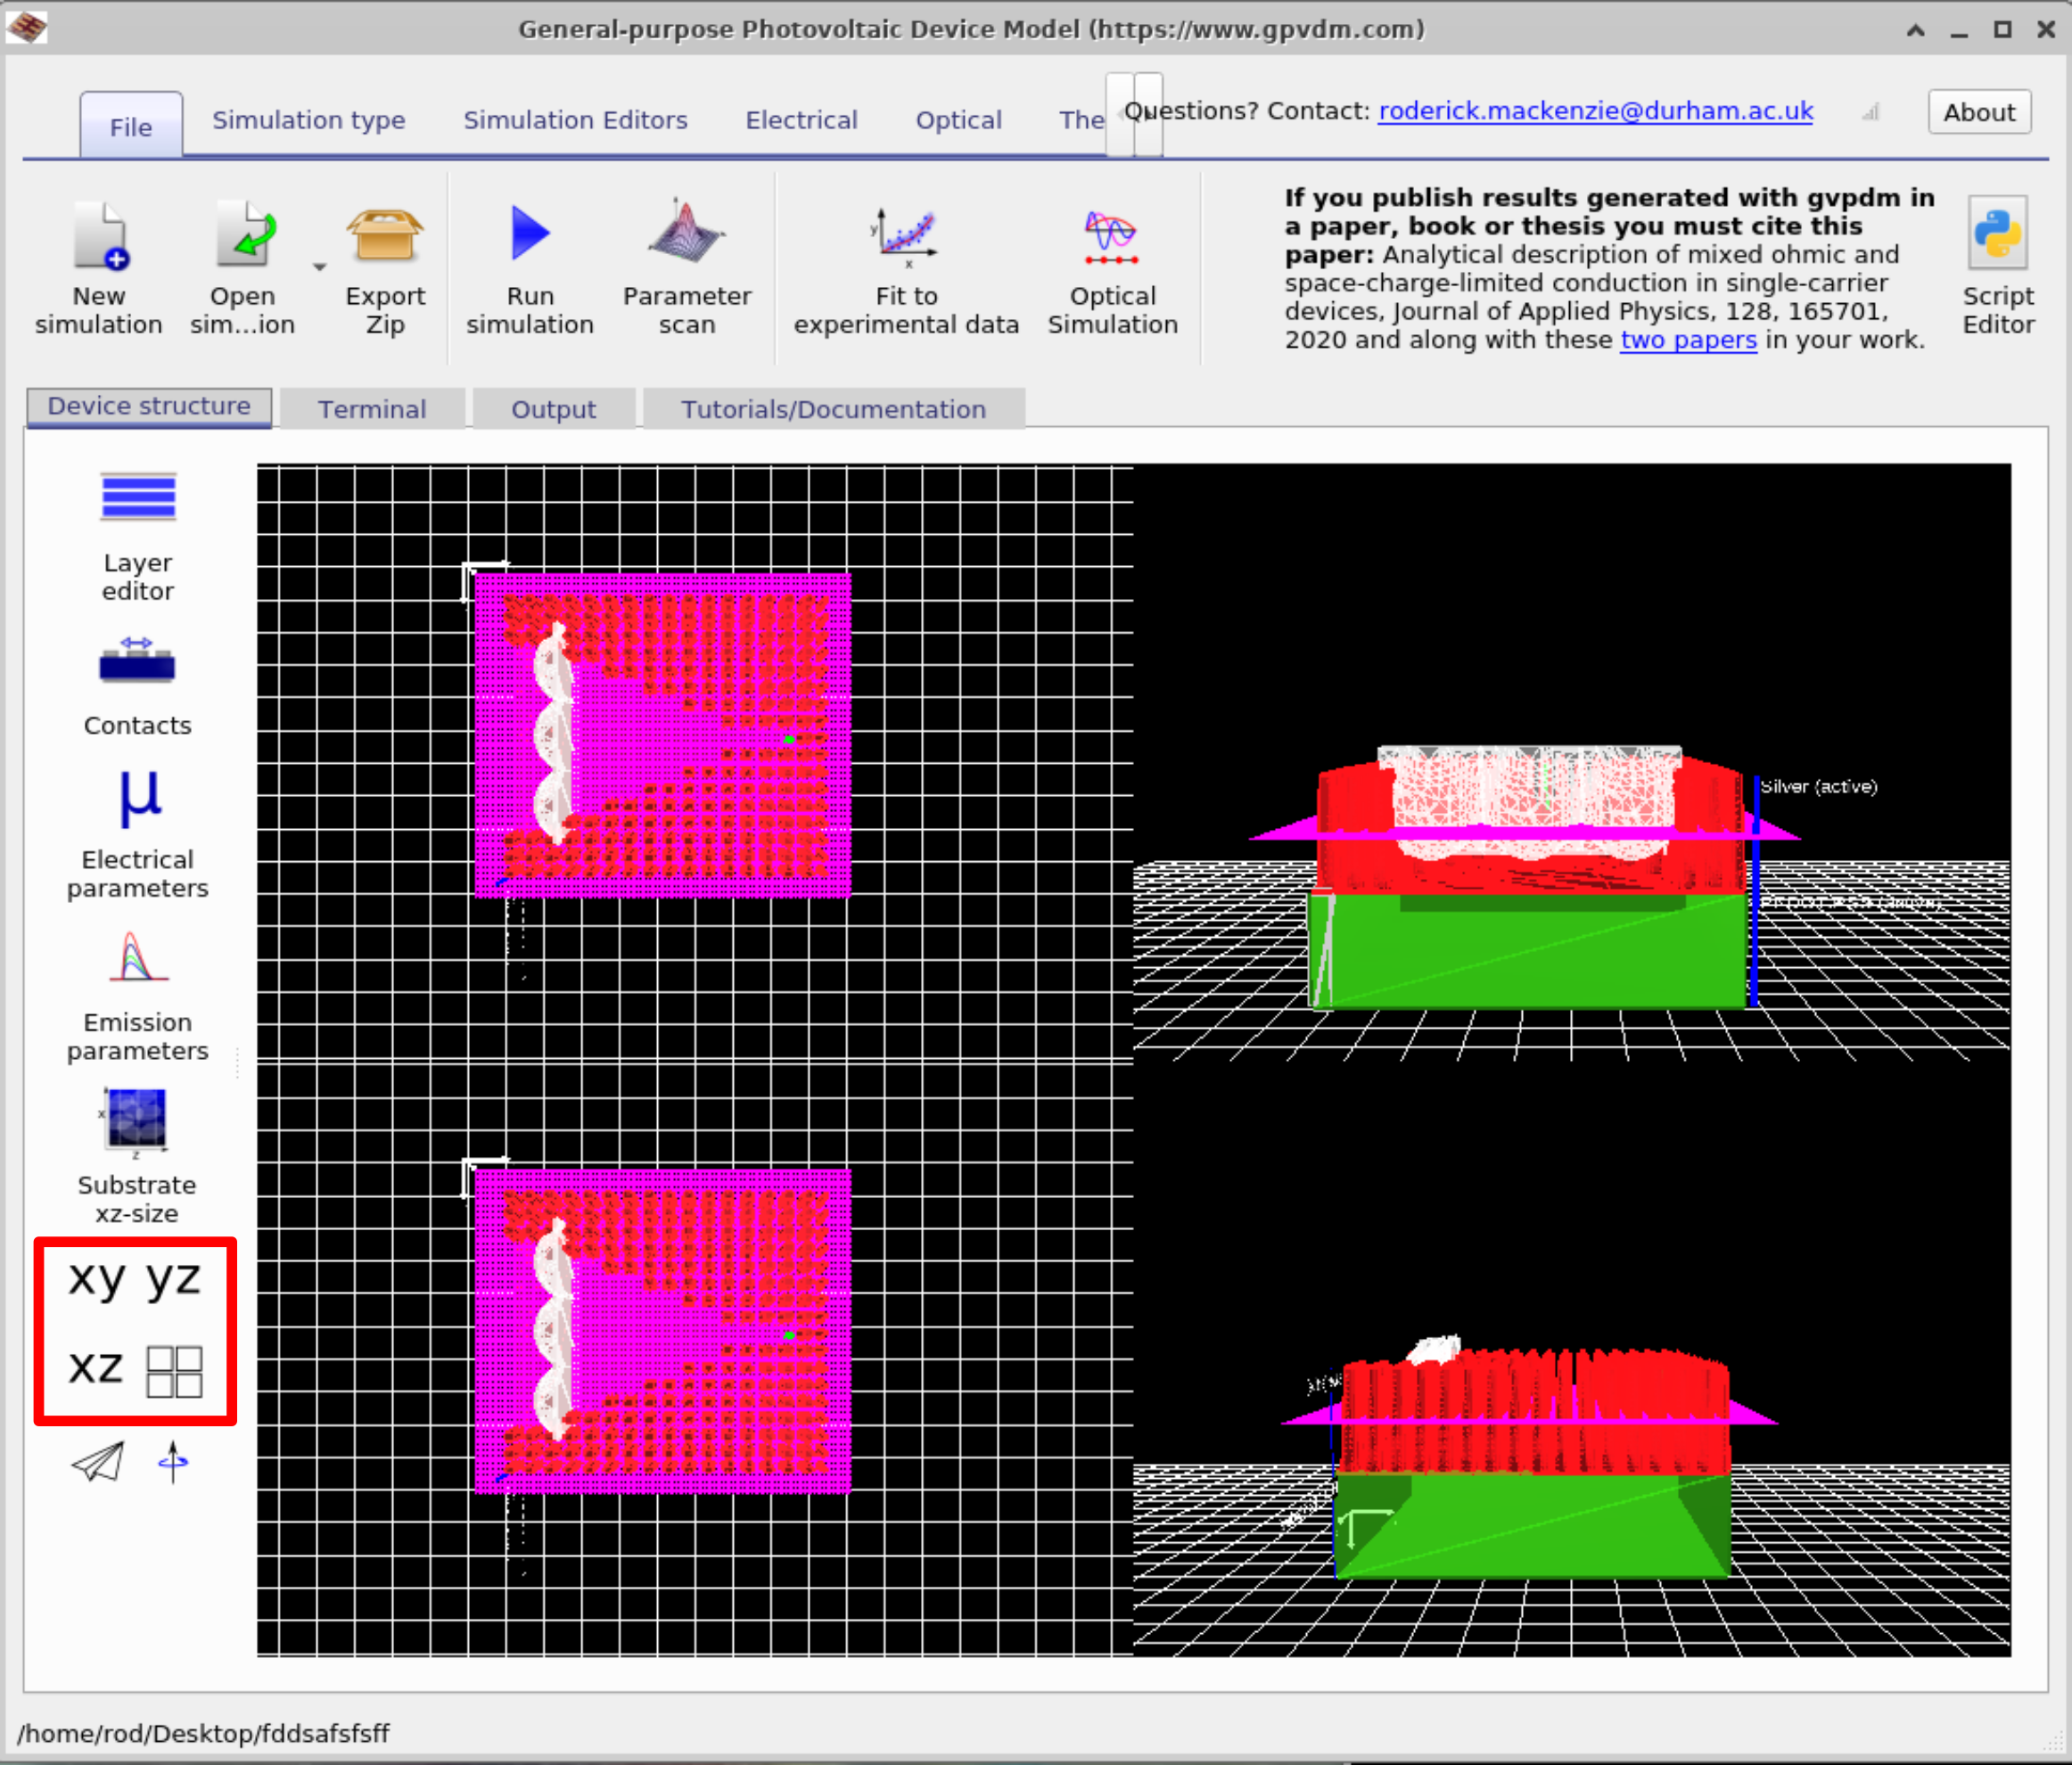
\includegraphics[width=0.7\textwidth]{./images/fdtd_7.png}
\caption{Changing the object view in gpvdm}
\label{fig:fdtdmainwindow}
\end{figure}

\begin{figure}[H]
\centering
\begin{tabular}{ c c }

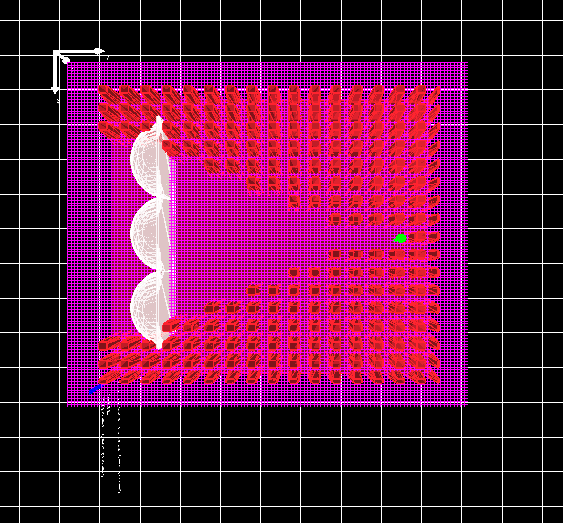
\includegraphics[width=0.5\textwidth,height=0.4\textwidth]{./images/fdtd_5.png}

&
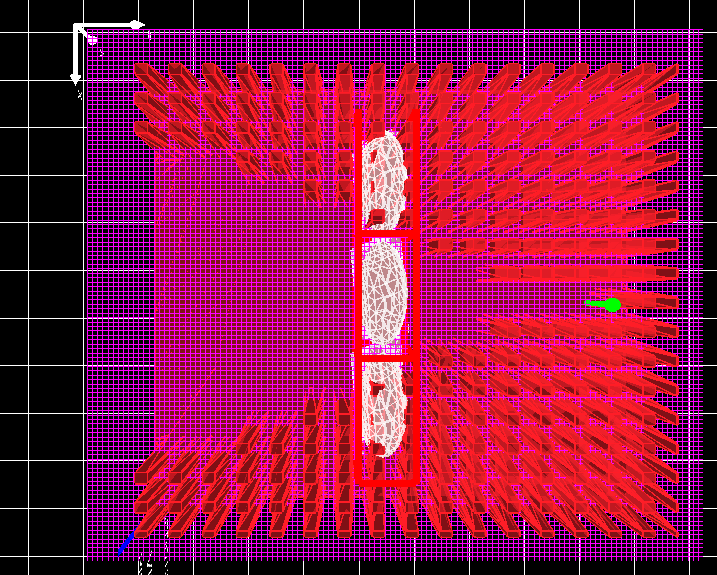
\includegraphics[width=0.5\textwidth,height=0.4\textwidth]{./images/fdtd_6.png}

\\

\end{tabular}
\caption{An example of moving objects in the simulation window.}
\label{fig:fdtdmovingobjects}
\end{figure}




\begin{figure}[H]
\centering
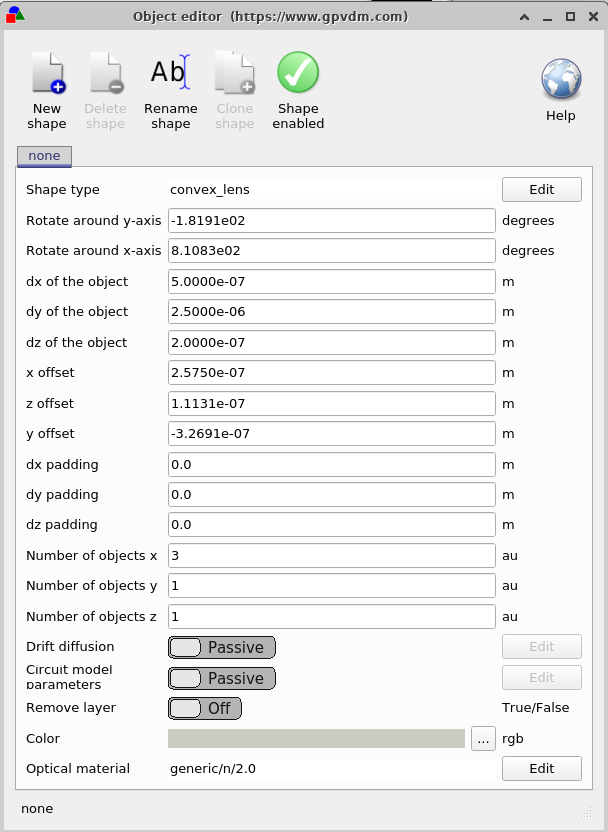
\includegraphics[width=0.7\textwidth]{./images/fdtd_12.png}
\caption{The object viewer. This window is brought up by right clicking on an object and selecting \emph{Edit}.}
\label{fig:objectviewer}
\end{figure}

\subsection{Manipulating light sources in gpvdm}
 Also visible in figure \ref{fig:fdtdmovingobjects} is the light source given by the green arrow. Try moving this more forward in the device.

\subsection{Theoretical background}
References for this section are \cite{FDTD_Schneider}. This section of the manual aims to describe the FDTD code in full with verbose derivations to help understanding/pick up errors.

Ampere’s law is given as  \cite{FDTD_Schneider}
\begin{equation}
\sigma  \boldsymbol{E} + \epsilon \frac{\partial  \boldsymbol{E}}{\partial t} = \nabla \times \boldsymbol{H} =
\begin{vmatrix} \hat{\boldsymbol{x}} & \hat{\boldsymbol{y}} & \hat{\boldsymbol{z}} \\ 
\frac{\partial}{\partial x} & \frac{\partial}{\partial y} & \frac{\partial}{\partial z} \\ 
H_{x} & H_{y} & H_{z}
\end{vmatrix}
\end{equation}


which can be expanded as

\begin{equation}
\sigma  E_{x} + \epsilon \frac{\partial  E_{x}}{\partial t} = \frac{\partial  H_{z}}{\partial y}-\frac{\partial  H_{y}}{\partial z}
\end{equation}

\begin{equation}
\sigma  E_{y} + \epsilon \frac{\partial  E_{y}}{\partial t} = -\frac{\partial  H_{z}}{\partial x}+\frac{\partial  H_{x}}{\partial z}
\end{equation}

\begin{equation}
\sigma  E_{z} + \epsilon \frac{\partial  E_{z}}{\partial t} = \frac{\partial  H_{y}}{\partial x}-\frac{\partial  H_{x}}{\partial y}
\end{equation}


For the case $\frac{\partial}{\partial y}=0$

\begin{equation}
\begin{split}
&\sigma  E_{x} + \epsilon \frac{\partial  E_{x}}{\partial t} =-\frac{\partial  H_{y}}{\partial z}\\
&\sigma  E_{y} + \epsilon \frac{\partial  E_{y}}{\partial t} = -\frac{\partial  H_{z}}{\partial x}+\frac{\partial  H_{x}}{\partial z}\\
&\sigma  E_{z} + \epsilon \frac{\partial  E_{z}}{\partial t} = \frac{\partial  H_{y}}{\partial x}
\end{split}
\end{equation}

for $E_{x}$
\begin{equation}
\begin{split}
&\sigma  E_{x} + \epsilon \frac{\partial  E_{x}}{\partial t} =-\frac{\partial  H_{y}}{\partial z}\\
&\sigma  \frac{E_{x}^{t+1}[]+E_{x}^{t}[]}{2} + \epsilon \frac{E_{x}^{t+1}[]-E_{x}^{t}[]}{\Delta t} = -\frac{H_{y}^{t+\frac{1}{2}}[\frac{1}{2}]-H_{y}^{t+\frac{1}{2}}[-\frac{1}{2}]}{\Delta z}\\
&\sigma  \frac{E_{x}^{t+1}[]}{2} + \epsilon \frac{E_{x}^{t+1}[]}{\Delta t} = -\frac{H_{y}^{t+\frac{1}{2}}[\frac{1}{2}]-H_{y}^{t+\frac{1}{2}}[-\frac{1}{2}]}{\Delta z}-\sigma  \frac{E_{x}^{t}[]}{2}+\epsilon \frac{E_{x}^{t}[]}{\Delta t}\\
&\sigma  \frac{E_{x}^{t+1}[]}{2} + \epsilon \frac{E_{x}^{t+1}[]}{\Delta t} = -\frac{H_{y}^{t+\frac{1}{2}}[\frac{1}{2}]-H_{y}^{t+\frac{1}{2}}[-\frac{1}{2}]}{\Delta z}-\sigma  \frac{E_{x}^{t}[]}{2}+\epsilon \frac{E_{x}^{t}[]}{\Delta t}\\
& \frac{\sigma \Delta t  + 2 \epsilon  }{ 2 \Delta t}E_{x}^{t+1}[] = -\frac{H_{y}^{t+\frac{1}{2}}[\frac{1}{2}]-H_{y}^{t+\frac{1}{2}}[-\frac{1}{2}]}{\Delta z}-\sigma  \frac{E_{x}^{t}[]}{2}+\epsilon \frac{E_{x}^{t}[]}{\Delta t}\\
& E_{x}^{t+1}[] = \left ( -\frac{H_{y}^{t+\frac{1}{2}}[\frac{1}{2}]-H_{y}^{t+\frac{1}{2}}[-\frac{1}{2}]}{\Delta z}-\sigma  \frac{E_{x}^{t}[]}{2}+\epsilon \frac{E_{x}^{t}[]}{\Delta t} \right ) \frac{2 \Delta t}{\sigma \Delta t  + 2 \epsilon}
\end{split}
\end{equation}

for $E_{y}$
\begin{equation}
\begin{split}
&\sigma  E_{y} + \epsilon \frac{\partial  E_{y}}{\partial t} = -\frac{\partial  H_{z}}{\partial x}+\frac{\partial  H_{x}}{\partial z}\\
&\sigma  \frac{E_{y}^{t+1}[]+E_{y}^{t}[]}{2} + \epsilon \frac{E_{y}^{t+1}[]-E_{y}^{t}[]}{\Delta t} = -\frac{H_{z}^{t+\frac{1}{2}}[\frac{1}{2}]-H_{z}^{t+\frac{1}{2}}[-\frac{1}{2}]}{\Delta x}+\frac{H_{x}^{t+\frac{1}{2}}[\frac{1}{2}]-H_{x}^{t+\frac{1}{2}}[-\frac{1}{2}]}{\Delta z}\\
&\sigma  \frac{E_{y}^{t+1}[]}{2} + \epsilon \frac{E_{y}^{t+1}[]}{\Delta t} = -\frac{H_{z}^{t+\frac{1}{2}}[\frac{1}{2}]-H_{z}^{t+\frac{1}{2}}[-\frac{1}{2}]}{\Delta x}+\frac{H_{x}^{t+\frac{1}{2}}[\frac{1}{2}]-H_{x}^{t+\frac{1}{2}}[-\frac{1}{2}]}{\Delta z}-\sigma \frac{E_{y}^{t}[]}{2} + \epsilon \frac{E_{y}^{t}[]}{\Delta t}\\
&E_{y}^{t+1}[] = \left ( -\frac{H_{z}^{t+\frac{1}{2}}[\frac{1}{2}]-H_{z}^{t+\frac{1}{2}}[-\frac{1}{2}]}{\Delta x}+\frac{H_{x}^{t+\frac{1}{2}}[\frac{1}{2}]-H_{x}^{t+\frac{1}{2}}[-\frac{1}{2}]}{\Delta z}-\sigma \frac{E_{y}^{t}[]}{2} + \epsilon \frac{E_{y}^{t}[]}{\Delta t} \right ) \frac{2 \Delta t}{\sigma \Delta t  + 2 \epsilon}
\end{split}
\end{equation}

for $E_{z}$
\begin{equation}
\begin{split}
&\sigma  E_{z} + \epsilon \frac{\partial  E_{z}}{\partial t} = \frac{\partial  H_{y}}{\partial x}\\
&\sigma  \frac{E_{z}^{t+1}[]+E_{z}^{t}[]}{2} + \epsilon \frac{E_{z}^{t+1}[]-E_{z}^{t}[]}{\Delta t} = \frac{H_{y}^{t+\frac{1}{2}}[\frac{1}{2}]-H_{y}^{t+\frac{1}{2}}[-\frac{1}{2}]}{\Delta x}\\
&\sigma  \frac{E_{z}^{t+1}[]}{2} + \epsilon \frac{E_{z}^{t+1}[]}{\Delta t} = \frac{H_{y}^{t+\frac{1}{2}}[\frac{1}{2}]-H_{y}^{t+\frac{1}{2}}[-\frac{1}{2}]}{\Delta x}-\sigma  \frac{E_{z}^{t}[]}{2} + \epsilon \frac{E_{z}^{t}[]}{\Delta t}\\
&E_{z}^{t+1}[]= \left ( \frac{H_{y}^{t+\frac{1}{2}}[\frac{1}{2}]-H_{y}^{t+\frac{1}{2}}[-\frac{1}{2}]}{\Delta x}-\sigma  \frac{E_{z}^{t}[]}{2} + \epsilon \frac{E_{z}^{t}[]}{\Delta t} \right ) \frac{2 \Delta t}{\sigma \Delta t  + 2 \epsilon}\\
\end{split}
\end{equation}

Faraday's law is given as \cite{FDTD_Schneider}
\begin{equation}
-\sigma_{m}  \boldsymbol{H} - \mu \frac{\partial  \boldsymbol{H}}{\partial t} = \nabla \times \boldsymbol{E} =
\begin{vmatrix} \hat{\boldsymbol{x}} & \hat{\boldsymbol{y}} & \hat{\boldsymbol{z}} \\ 
\frac{\partial}{\partial x} & \frac{\partial}{\partial y} & \frac{\partial}{\partial z} \\ 
E_{x} & E_{y} & E_{z}
\end{vmatrix}
\end{equation}

which can be expanded to give:

\begin{equation}
-\sigma_{m}  H_{x} - \mu \frac{\partial  H_{x}}{\partial t} = \frac{\partial  E_{z}}{\partial y}-\frac{\partial  E_{y}}{\partial z}
\end{equation}

\begin{equation}
-\sigma_{m}  H_{y} - \mu \frac{\partial  H_{y}}{\partial t} = -\frac{\partial  E_{z}}{\partial x}+\frac{\partial  E_{x}}{\partial z}
\end{equation}

\begin{equation}
-\sigma_{m}  H_{z} - \mu \frac{\partial  H_{z}}{\partial t} = \frac{\partial  E_{y}}{\partial x}-\frac{\partial  E_{x}}{\partial y}
\end{equation}

With $\sigma_m=0$ and $\frac{\partial}{\partial y}=0$

\begin{equation}
\begin{split}
  &\frac{\partial  H_{x}}{\partial t} = \frac{1}{\mu} \left ( \frac{\partial  E_{y}}{\partial z} \right )\\
  &\frac{\partial  H_{y}}{\partial t} = \frac{1}{\mu} \left ( \frac{\partial  E_{z}}{\partial x}-\frac{\partial  E_{x}}{\partial z} \right )\\
  &\frac{\partial  H_{z}}{\partial t} = - \frac{1}{\mu} \left ( \frac{\partial  E_{y}}{\partial x} \right )
\end{split}
\end{equation}


which discretizing gives

\begin{equation}
\begin{split}
  & H_{x}^{t+1} = \frac{1}{\mu} \left ( \frac{E_{y}^{t+\frac{1}{2}}[\frac{1}{2}]-E_{y}^{t+\frac{1}{2}}[-\frac{1}{2}]}{\Delta z} \right ) \Delta t + H_{x}^{t}[]\\
  & H_{y}^{t+1} = \frac{1}{\mu} \left ( \frac{E_{z}^{t+\frac{1}{2}}[\frac{1}{2}]-E_{z}^{t+\frac{1}{2}}[-\frac{1}{2}]}{\Delta x}-\frac{E_{x}^{t+\frac{1}{2}}[\frac{1}{2}]-E_{x}^{t+\frac{1}{2}}[-\frac{1}{2}]}{\Delta z} \right ) \Delta t+ H_{y}^{t}[]\\
  & H_{z}^{t+1} =  \frac{1}{\mu} \left ( - \frac{E_{y}^{t+\frac{1}{2}}[\frac{1}{2}]-E_{y}^{t+\frac{1}{2}}[-\frac{1}{2}]}{\Delta x} \right ) \Delta t + H_{x}^{z}[]
\end{split}
\end{equation}
